\documentclass[a4paper,12pt]{article}
\usepackage[a4paper,margin=1in]{geometry}
\usepackage{graphicx}
\usepackage{hyperref}
\usepackage{float}
\usepackage{xurl} % Added for better URL line breaking
\usepackage[htt]{hyphenat} % Added for hyphenation in tt environments
\usepackage{fancyhdr}
\usepackage{ragged2e} % Added for improved ragged right
\usepackage{graphicx}
\usepackage{caption}
\usepackage{subcaption}

% Header/Footer
\newcommand{\changefont}{%
    \fontsize{5}{11}\selectfont
}
\pagestyle{fancy}
\fancyhead[L]{\changefont CSE364 - Operating Systems Course - Project Report}
\fancyfoot[C]{\thepage}

\setlength{\emergencystretch}{3em} % Added to help with line breaking

\begin{document}
\sloppy % Added to allow more flexible line breaking

% Title Page
\begin{titlepage}
\centering
\vspace{1cm}
{
\begin{figure}
    \centering
    
\includegraphics[width=1\linewidth]{logo.png}
    \label{fig:enter-label}
\end{figure}


 \textbf{\\[2cm]MSA Univeristy -- Faculty of Engineering \\[1cm]  Computer Systems Engineering \\[1cm]
 }

\LARGE \textbf{Restaurant Order Scheduling System}}\\[1.5cm]
\textbf{Course:} CSE364 - Operating Systems\\
\textbf{Instructor:} Dr. Ahmed Ayoub\\[1cm]
\textbf{Team Members:}\\
Ahmed Essam Mohamed (236385)\\
Mohamed Ali Saafan (238521)\\ 
Pierre Ramez Francis (237563)\\
Ahmed Mohammed Elsayed (238057)\\ [1cm]

\textbf{Submission Date:} \today\\[2cm]
\vfill
\end{titlepage}

% Table of Contents
\tableofcontents
\newpage

% Section 1: Introduction
\section{Introduction}
\begin{itemize}
    \item Brief description of the project: This project, titled "Restaurant Order Scheduling System," focuses on developing an operating system-based task scheduler. The primary goal is to optimize the processing of restaurant orders, thereby minimizing customer wait times. The system will leverage key OS concepts such as process scheduling, multi-threading, and priority queues to achieve efficient order management.
    \item The problem statement and its relevance: In a busy restaurant environment, inefficient order processing can lead to increased customer wait times, dissatisfaction, and potential loss of business. This project addresses the challenge of managing a high volume of orders with varying complexities and priorities. The relevance lies in applying OS scheduling principles to a real-world scenario to improve service delivery and operational efficiency in the food service industry.
    \item Objectives and expected outcomes: The main objective is to design and implement a scheduling system that dynamically prioritizes and processes orders to reduce average and maximum wait times. Expected outcomes include a functional scheduler capable of handling concurrent orders, a comparative analysis of different scheduling algorithms (e.g., FCFS, Priority, Round Robin), and a demonstration of improved performance metrics compared to a baseline or simpler scheduling approach.
\end{itemize}
\newpage

 % Section 2: Background & Related Work
\section{Background and Related Work}
\begin{itemize}
    \item Overview of relevant OS concepts:
        \begin{itemize}
            \item \textbf{Process Scheduling:} This is a fundamental OS function that determines which process runs when multiple processes are competing for CPU time. Common algorithms include First-Come, First-Served (FCFS), Round Robin (RR), Shortest Job First (SJF), and Priority Scheduling. This project explores FCFS, RR, and Priority Scheduling to manage restaurant orders as processes.
            \item \textbf{Multi-threading:} Multi-threading allows a single process to manage multiple tasks concurrently. In this project, multi-threading is employed to handle incoming orders, process them according to the selected scheduling algorithm, and update the UI without blocking, simulating a responsive and efficient system.
            \item \textbf{Priority Queues:} A priority queue is an abstract data type where each element has an associated priority. Elements with higher priorities are served before elements with lower priorities. This project utilizes priority queues in the Priority Scheduling algorithm, where orders might be prioritized based on factors like order size, customer type, or preparation time.
        \end{itemize}
\end{itemize}
\newpage

% Section 3: System Design & Methodology
\section{System Design and Methodology}
\RaggedRight % Changed from \raggedright
\begin{itemize}
    \item System architecture with diagrams:
        \begin{itemize}
            \item The system is designed as a C++ application. 
            \item It utilizes a graphical user interface (GUI) built with ImGui to visualize the scheduling process and allow user interaction.
            \item GLFW is used for window creation and management.
            \item The core logic is separated into classes representing Orders, Menu Items, and different Schedulers (FCFS, Round Robin, Priority Queue).
            \item Multi-threading is employed to ensure the GUI remains responsive while schedulers process orders in the background.
            
        \end{itemize}
    \item Technologies and tools used:
        \begin{itemize}
            \item Programming Language: C++ (Standard: C++17)
            \item GUI Library: Dear ImGui (imgui)
            \item Windowing and Input: GLFW
            \item Build System: CMake
            \item Key Data Structures: \nolinkurl{std::deque} for queues, \nolinkurl{std::vector} for collections, \nolinkurl{std::mutex} and \nolinkurl{std::condition_variable} for thread synchronization.
        \end{itemize}
    \item Description of key algorithms:
        \begin{itemize}
            \item \textbf{First-Come, First-Served (FCFS):} Orders are processed strictly in the order they are received. A single queue (\nolinkurl{std::deque<Order>}) is maintained. The \nolinkurl{FCFS::processOrders()} method retrieves orders from the front of the queue and simulates their processing.
            \item \textbf{Round Robin (RR):} Orders are processed in a cyclic manner, each for a fixed time quantum. If an order is not completed within its time quantum, it is moved to the end of the queue. The \nolinkurl{RR::processOrders()} method implements this logic, managing remaining processing time for each order.
            \item \textbf{Priority Queue (PQ):} Orders are assigned a priority (e.g., based on preparation time or a VIP status). Higher priority orders are processed before lower priority ones. This implementation uses two queues: one for high-priority orders and one for low-priority orders (\nolinkurl{PriorityScheduler::highPriorityQueue}, \nolinkurl{PriorityScheduler::lowPriorityQueue}). The \nolinkurl{PriorityScheduler::processOrders()} method prioritizes the high-priority queue and can preempt low-priority orders if a high-priority order arrives.
            \item \textbf{Order Management:} The \nolinkurl{Order} class encapsulates details like item name, preparation time, and status. The \nolinkurl{Menu} class manages available items.
            \item \textbf{Concurrency:} Each scheduling algorithm runs in its own thread (\nolinkurl{std::thread}) to allow simultaneous operation and comparison. Mutexes (\nolinkurl{std::mutex}) and condition variables (\nolinkurl{std::condition_variable}) are used to protect shared data structures (the order queues) and manage thread synchronization.
        \end{itemize}
\end{itemize}
\newpage

% Section 4: Implementation and Challenges
\section{Implementation and Challenges}
\RaggedRight % Changed from \raggedright
\begin{itemize}
    \item Code structure and major functions:
        \begin{itemize}
            \item The project is organized into several C++ classes, primarily within the \nolinkurl{src} directory, each responsible for a specific aspect of the system:
                \begin{itemize}
                    \item \nolinkurl{main.cpp}: The main entry point of the application. It initializes and runs the Command Line Interface (CLI) in a separate thread and starts the Graphical User Interface (GUI) main loop.
                    \item \nolinkurl{GUI.cpp/h}: Manages the graphical user interface using Dear ImGui, GLFW, and Vulkan. It's responsible for rendering all UI elements, including the menu, scheduler queues, and performance metrics. Key functions include \nolinkurl{main_loop()} for the primary event and rendering cycle, and various setup functions for Vulkan and ImGui.
                    \item \nolinkurl{Application.cpp/h}: Acts as a central coordinator for the UI logic. It initializes scheduler instances (\nolinkurl{FCFS}, \nolinkurl{RR}, \nolinkurl{PriorityScheduler}), provides functions to render different parts of the UI like \nolinkurl{MenuPicker()}, \nolinkurl{SchedQueues()}, and \nolinkurl{RenderCompletedOrdersWindow()}, and handles interactions like adding orders from the menu to the schedulers.
                    \item \nolinkurl{CLI.cpp/h}: Provides a command-line interface for interacting with the system, primarily for adding orders or testing. The \nolinkurl{init()} function sets up the CLI environment and can be used to script order additions.
                    \item \nolinkurl{Order.cpp/h}: Defines the \nolinkurl{Order} class, which encapsulates all properties of a restaurant order, such as \nolinkurl{pid} (order ID), \nolinkurl{itemName}, \nolinkurl{prepTime} (burst time), \nolinkurl{remainingTime}, \nolinkurl{priority}, \nolinkurl{arrivalTime}, \nolinkurl{waitingTime}, and \nolinkurl{turnaroundTime}. It also includes methods to get and modify these attributes.
                    \item \nolinkurl{MenuItem.h} and \nolinkurl{Menu.cpp/h}: Define \nolinkurl{MenuItem} (representing an item that can be ordered) and \nolinkurl{Menu} (a collection of \nolinkurl{MenuItem}s). \nolinkurl{Menu} class provides functionality to display items and retrieve them by ID.
                    \item \nolinkurl{FCFS.cpp/h}: Implements the First-Come, First-Served scheduling algorithm. Major functions include \nolinkurl{addOrder()} to add an order to its queue, \nolinkurl{processOrders()} which runs in a separate thread to process orders sequentially, \nolinkurl{start()}/\nolinkurl{stop()} to control the processing thread, and static methods like \nolinkurl{getQueue()}, \nolinkurl{getCurrentlyProcessingOrder()}, and \nolinkurl{getCompletedOrders()} for UI display.
                    \item \nolinkurl{RR.cpp/h}: Implements the Round Robin scheduling algorithm with a configurable time quantum. Similar to FCFS, it has \nolinkurl{addOrder()}, \nolinkurl{processOrders()} (which handles time slicing and re-queuing), \nolinkurl{start()}/\nolinkurl{stop()}, and static methods for UI data retrieval.
                    \item \nolinkurl{PQ.cpp/h}: Implements a Priority-based preemptive scheduling algorithm. It maintains separate queues for high and low priority orders (determined by \nolinkurl{PRIORITY_THRESHOLD} on preparation time). Key functions include \nolinkurl{addOrder()} (which places orders in the appropriate priority queue), \nolinkurl{processOrders()} (which prioritizes high-priority tasks and can preempt lower-priority ones), \nolinkurl{start()}/\nolinkurl{stop()}, and static methods for UI data.
                    \item \nolinkurl{States.h}: Defines an enumeration \nolinkurl{ProcessState} (e.g., \nolinkurl{NEW}, \nolinkurl{READY}, \nolinkurl{RUNNING}, \nolinkurl{TERMINATED}, \nolinkurl{WAITING}) likely used by the \nolinkurl{Order} class to track its current status, although direct usage in schedulers might be implicit.
                    \item \nolinkurl{Timer.cpp/h}: A utility class responsible for calculating and storing performance metrics like waiting time and turnaround time for each order and for each scheduler. It has functions like \nolinkurl{startwaitTimer()}, \nolinkurl{stopwaitTimer()}, \nolinkurl{calcualteWaitTimer()}, \nolinkurl{startTurnaroundTimer()}, \nolinkurl{stopTurnaroundTimer()}, and \nolinkurl{calculateTurnaroundTime()}.
                \end{itemize}
        \end{itemize}
    \item Problems faced and solutions:
        \begin{itemize}
            \item \textbf{Concurrency Management:} A key challenge was managing concurrent access to shared order queues by multiple scheduler threads and the main thread (for adding orders via GUI/CLI). This was addressed by using \nolinkurl{std::mutex} to protect critical sections where queues are modified or accessed, and \nolinkurl{std::condition_variable} to signal worker threads when new orders are available or when processing should stop. Each scheduler (\nolinkurl{FCFS}, \nolinkurl{RR}, \nolinkurl{PQ}) runs its \nolinkurl{processOrders()} loop in a separate \nolinkurl{std::thread}.
            \item \textbf{GUI Responsiveness:} To prevent the GUI from freezing while orders are being processed, the scheduling logic for each algorithm was offloaded to separate threads. The GUI thread then polls data from these schedulers (e.g., current order, upcoming queue, completed orders) using thread-safe static methods.
            \item \textbf{Accurate Performance Metrics:} Calculating waiting and turnaround times accurately, especially for preemptive schedulers like Round Robin and Priority Queue, requires careful state and time tracking. The \nolinkurl{Timer} class was implemented to encapsulate this logic, associating timers with individual orders and specific scheduler types to ensure correct calculations upon order completion or preemption.
            \item \textbf{State Management for Orders:} Orders transition through various states (e.g., new, processing, completed). The \nolinkurl{Order} class attributes (like \nolinkurl{remainingTime}) and the scheduler logic implicitly manage these states. For instance, an order's \nolinkurl{remainingTime} is reduced, and it's either re-queued (in RR) or moved to completed orders.
            \item \textbf{Algorithm Implementation Details:} Implementing the nuances of each scheduling algorithm (e.g., time quantum handling in RR, preemption logic in PQ, correct queue management) required careful design. For example, the Priority Scheduler uses two distinct queues and logic to check for high-priority arrivals to preempt lower-priority tasks.
            \item \textbf{User Interface Design:} Presenting complex information from three concurrent schedulers in an understandable way was a UI challenge. The \nolinkurl{Application.cpp} uses ImGui's features (columns, child windows, tables) to display the state of each scheduler, the menu, and the completed orders with their metrics in a structured manner.
        \end{itemize}
\end{itemize}
\newpage

% Section 5: Testing and Results
\section{Testing and Results}
\RaggedRight % Changed from \raggedright
\begin{itemize}
    \item Testing strategies and sample test cases: 

                \begin{itemize}
                    \item Test Case 1 (FCFS): Add 3 orders with varying prep times. Verify completion order and times.
                    \item Test Case 2 (RR): Add 2 long orders and 1 short order. Verify time slicing and completion.
                    \item Test Case 3 (PQ): Add high and low priority orders. Verify preemption and prioritization.
                \end{itemize}
    \item Performance analysis (if applicable):
        \begin{itemize}
           The program results shows all three schedulers working correctly, where FCFS works in a first come first serve non-preemptive manner, Round Robin works on each order for a time quantum of 6 units and the Priority Queue scheduler places orders of burst time < 6 in a high priority queue to preempt the currently scheduled orders to work on them first.
        \end{itemize}
    \item Screenshots or tables of results:
\begin{figure}[H]
    \centering
    \begin{subfigure}[b]{0.32\linewidth}
        \centering
        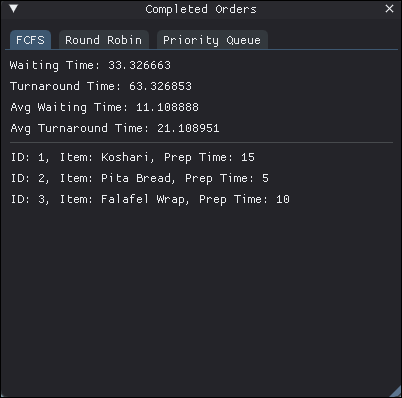
\includegraphics[width=\linewidth]{FCFS.png}
        \caption{FCFS}
        \label{fig:FCFS}
    \end{subfigure}
    \hfill
    \begin{subfigure}[b]{0.32\linewidth}
        \centering
        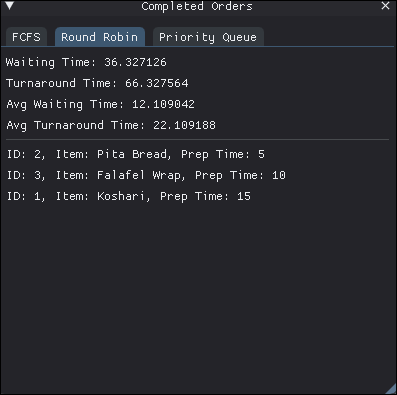
\includegraphics[width=\linewidth]{RR.png}
        \caption{Round Robin}
        \label{fig:RR}
    \end{subfigure}
    \hfill
    \begin{subfigure}[b]{0.32\linewidth}
        \centering
        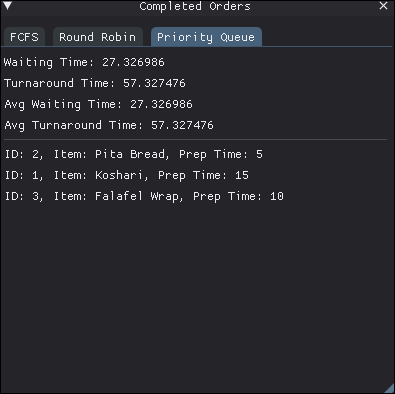
\includegraphics[width=\linewidth]{PQ.png}
        \caption{Priority Queue}
        \label{fig:PQ}
    \end{subfigure}
    \caption{Different Scheduling Algorithms Results}
    \label{fig:gui-all}
\end{figure}
\end{itemize}
\newpage

% Section 6: Conclusion and Future Work
\section{Conclusion and Future Work}
\begin{itemize}
    \item Summary of findings:
        \begin{itemize}
            \item This project successfully developed a "Restaurant Order Scheduling System" that implements and visualizes three common CPU scheduling algorithms: First-Come, First-Served (FCFS), Round Robin (RR), and Priority Queue (PQ).
            \item The system utilizes C++ for its core logic, Dear ImGui for the graphical user interface, and GLFW for window management, providing a platform to observe the behavior of these algorithms in a simulated restaurant environment.
            \item Multi-threading was employed to ensure that the GUI remains responsive while the scheduling algorithms process orders in the background, demonstrating a key operating system concept for concurrent processing.
            \item The implementation effectively simulates order management, processing, and the calculation of basic performance metrics like waiting time and turnaround time for each scheduler.
        \end{itemize}
    \item Suggested improvements and next steps:
        \begin{itemize}
            \item \textbf{Enhance Performance Measurement:} A key area for future work is the refinement of performance metric collection. The current methods for calculating waiting and turnaround times can be influenced by the overhead of context switching between threads and GUI updates. More precise timing mechanisms, potentially isolated from the GUI thread or using more sophisticated profiling tools, could yield more accurate performance data.
            \item \textbf{Advanced Priority Criteria:} The Priority Queue scheduler could be enhanced with more dynamic or complex priority assignment rules, such as considering order value, customer loyalty status, or adaptive priorities based on current queue lengths.
            \item \textbf{Additional Scheduling Algorithms:} Implement and compare other scheduling algorithms like Shortest Job First (SJF) or Shortest Remaining Time First (SRTF), which might offer different performance trade-offs.
            \item \textbf{Dynamic Time Quantum for RR:} Allow the time quantum for the Round Robin scheduler to be dynamically adjusted or optimized based on system load or order characteristics.
            \item \textbf{Persistent Storage:} Implement saving and loading of menu configurations or order histories.
            \item \textbf{Networked Operation:} Extend the system to support order entry from multiple clients over a network, simulating a more realistic restaurant setup.
            \item \textbf{More Detailed Simulation:} Incorporate more realistic simulation aspects, such as varying chef availability or kitchen resource contention.
        \end{itemize}
\end{itemize}
\newpage

% Section 7: References
\section{References}
\begin{itemize}
    \item Silberschatz, A., Galvin, P. B., & Gagne, G. (2018). \textit{Operating system concepts}. Wiley.
    \item C++ Standard Library Documentation. (e.g., \url{https://en.cppreference.com/w/cpp})
    \item Dear ImGui Library. (e.g., \url{https://github.com/ocornut/imgui})
    \item GLFW Library. (e.g., \url{https://www.glfw.org/})
\end{itemize}
\newpage
% Appendices (if needed)
\appendix
\section{Appendix A: Additional Materials}
\begin{itemize}
    \item GUI presentation:
    \begin{figure}[H] % Forces the figure to appear "Here"
        \centering
        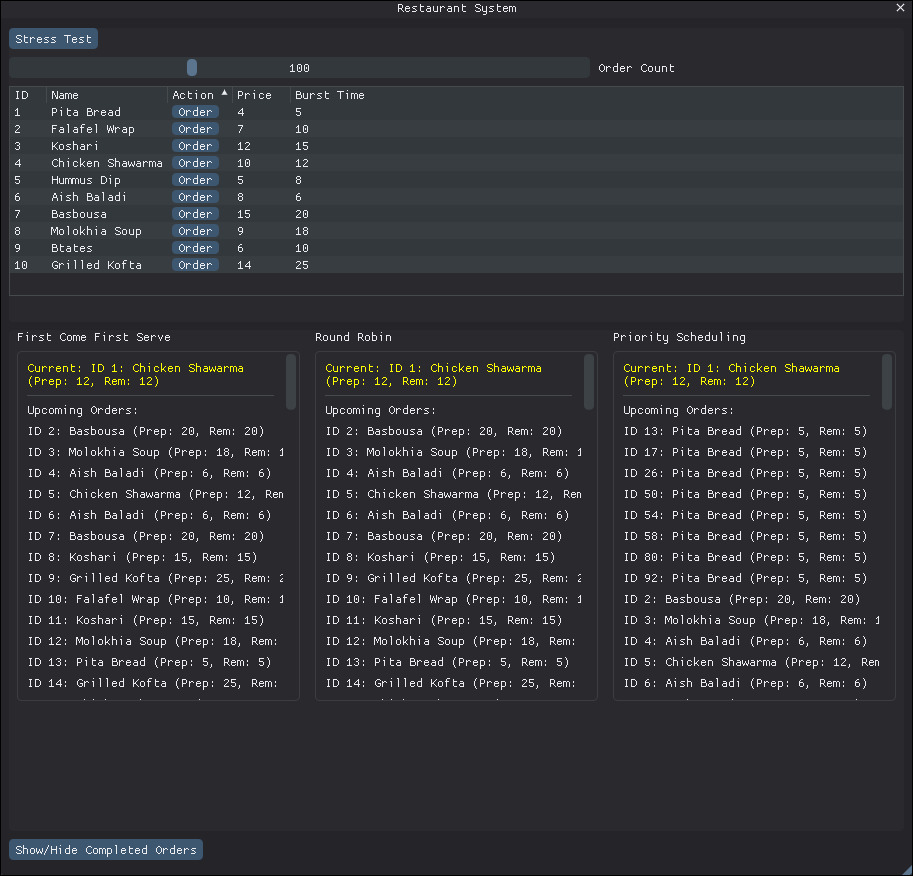
\includegraphics[width=1\linewidth]{GUI.jpeg}
        \caption{GUI presentation} % Optional: add a caption
        \label{fig:gui-presentation}
    \end{figure}
\end{itemize}


\newpage
% --- Key Code Snippets: Readable and Presentable Format ---

\subsection*{Key Code Snippets}
Below are representative code snippets from the implementation to illustrate the core classes and algorithms of the Restaurant Order Scheduling System. These are provided for technical context and are not exhaustive. Each snippet is accompanied by a brief description for clarity.

\begin{verbatim}
// Example from FCFS::addOrder()
void FCFS::addOrder(Order& order) {
    {
        std::lock_guard<std::mutex> lock(queueMutex); // Protects orderQueue
        orderQueue.push_back(order);
        // ...
    }
    cv.notify_one(); 
}
    \end{verbatim}

\begin{verbatim}
// From Application::MenuPicker() when ordering an item
Order newOrder(item);
fcfs_scheduler.addOrder(newOrder);
rr_scheduler.addOrder(newOrder);
priority_scheduler_instance.addOrder(newOrder);
    \end{verbatim}

\begin{verbatim}
// Example from FCFS::start()
void FCFS::start() {
    std::lock_guard<std::mutex> lock(queueMutex); 
    if (threadStarted) return; 
    threadStarted = true;
    
    std::thread processingThread(&FCFS::processOrders, this);
    processingThread.detach(); 
}
\end{verbatim}

\begin{verbatim}
// From PriorityScheduler::addOrder(const Order& order)
void PriorityScheduler::addOrder(const Order& order) {
    std::string queueType; // For logging, not shown here
    {
        std::lock_guard<std::mutex> lock(queueMutex); 
        if (order.getPrepTime() < PRIORITY_THRESHOLD) {
            highPriorityQueue.push_back(order);
            timer.startwaitTimer(highPriorityQueue.back(), schedulerType);
            timer.startTurnaroundTimer(highPriorityQueue.back(), schedulerType);
        } else {
            lowPriorityQueue.push_back(order);
            timer.startwaitTimer(lowPriorityQueue.back(), schedulerType);
            timer.startTurnaroundTimer(lowPriorityQueue.back(), schedulerType);
        }
    }
    cv.notify_one(); 
}
\end{verbatim}

\begin{verbatim}
// From FCFS::processOrders()
void FCFS::processOrders() {
    isProcessing = true;
    while (isProcessing || !orderQueue.empty()) {
        Order localCurrentOrder;
        bool orderFound = false;
        {
            std::unique_lock<std::mutex> lock(queueMutex);
            cv.wait(lock, [this](){ return !orderQueue.empty() || !isProcessing; });
            
            if (!isProcessing && orderQueue.empty()) break;
            if (orderQueue.empty()) continue;

            localCurrentOrder = orderQueue.front();
            orderQueue.pop_front();
            orderFound = true;
        }

        if (orderFound) {
            { // Set currently processing order
                std::lock_guard<std::mutex> currentLock(s_currentOrderMutex);
                s_currentlyProcessingOrder = localCurrentOrder;
            }
            
            timer.stopwaitTimer(localCurrentOrder, schedulerType);
            sleep_for(seconds(localCurrentOrder.getPrepTime())); // Simulate processing
            timer.calcualteWaitTimer(localCurrentOrder, schedulerType);
            
            timer.stopTurnaroundTimer(localCurrentOrder, schedulerType);
            timer.calculateTurnaroundTime(localCurrentOrder, schedulerType);

            { // Add to completed orders
                std::lock_guard<std::mutex> lock(s_completedOrdersMutex);
                s_completedOrders.push_back(localCurrentOrder);
                Timer::endTimesSizes[FCFS_]++;
            }

            { // Clear currently processing order
                std::lock_guard<std::mutex> currentLock(s_currentOrderMutex);
                s_currentlyProcessingOrder.reset();
            }
        }
    }
}
\end{verbatim}
    

\end{document}
